\documentclass[aspectratio=169,10pt]{beamer}
% ---------------------------------------------------------------
% R3.07 SQL dans un langage de programmation -- preambule commun des diapositives
% Charte derivee de R5.A.08 Qualite de developpement (metropolis, dark tech)
% Palette IUT partagee (violet du logo + accent or)
% Utilisation :
%   \documentclass[aspectratio=169,10pt]{beamer}
%   % ---------------------------------------------------------------
% R3.07 SQL dans un langage de programmation -- preambule commun des diapositives
% Charte derivee de R5.A.08 Qualite de developpement (metropolis, dark tech)
% Palette IUT partagee (violet du logo + accent or)
% Utilisation :
%   \documentclass[aspectratio=169,10pt]{beamer}
%   % ---------------------------------------------------------------
% R3.07 SQL dans un langage de programmation -- preambule commun des diapositives
% Charte derivee de R5.A.08 Qualite de developpement (metropolis, dark tech)
% Palette IUT partagee (violet du logo + accent or)
% Utilisation :
%   \documentclass[aspectratio=169,10pt]{beamer}
%   \input{../../latex/common/r307-slides-preamble.tex}
%   \graphicspath{{../../latex/common/assets/}{img/}{figs/}}
% ---------------------------------------------------------------
\usetheme{metropolis}
\usepackage{appendixnumberbeamer}

\usepackage[T1]{fontenc}
\usepackage[utf8]{inputenc}
\usepackage[french]{babel}
\usepackage[scale=0.94]{tgheros}
\renewcommand{\familydefault}{\sfdefault}
\usepackage{amsmath,amssymb,amsfonts}
\usepackage{graphicx}
\usepackage{booktabs}
\usepackage{multirow}
\usepackage{tikz}
\usetikzlibrary{shapes.geometric, shapes, arrows, arrows.meta, positioning, calc, fit}
\usepackage{xcolor}
\usepackage{listings}
\usepackage[skins,listings]{tcolorbox}
\usepackage{qrcode}
\usepackage{hyperref}

% ---------------------------------------------------------------
% PALETTE (dark-mode tech: near-black canvas, violet (logo IUT) + gold accents)
% ---------------------------------------------------------------
\definecolor{qabg}{HTML}{0E1016}      % canvas background
\definecolor{qapanel}{HTML}{181B24}   % card / block panel
\definecolor{qapanelalt}{HTML}{20242F}% secondary panel tint
\definecolor{qaline}{HTML}{2B303D}    % hairline rules / table rules
\definecolor{qatext}{HTML}{ECEEF2}    % primary text (off-white)
\definecolor{qamuted}{HTML}{8B93A6}   % secondary / caption text
\definecolor{qaaccent}{HTML}{D93ED7}  % primary accent -- violet du logo IUT, eclairci pour fond sombre
\definecolor{qaaccent2}{HTML}{F2B84B} % secondary accent -- or/ambre
\definecolor{qacodekw}{HTML}{C792EA}  % code : mots-cles
\definecolor{qacodestr}{HTML}{C3E88D} % code : chaines
\definecolor{qacodecom}{HTML}{7F8AA3} % code : commentaires
\definecolor{qacodeann}{HTML}{F2B84B} % code : annotations / javadoc

\setbeamercolor{background canvas}{bg=qabg}
\setbeamercolor{normal text}{fg=qatext}
\setbeamercolor{palette primary}{bg=qabg, fg=qamuted}
\setbeamercolor{frametitle}{bg=qabg, fg=qatext}
\setbeamercolor{progress bar}{fg=qaaccent, bg=qaline}
\setbeamercolor{alerted text}{fg=qaaccent2}
\setbeamercolor{block title}{bg=qapanel, fg=qaaccent}
\setbeamercolor{block body}{bg=qapanel, fg=qatext}
\setbeamercolor{block title alerted}{bg=qapanel, fg=qaaccent2}
\setbeamercolor{block body alerted}{bg=qapanel, fg=qatext}
\setbeamercolor{block title example}{bg=qapanelalt, fg=qaaccent}
\setbeamercolor{block body example}{bg=qapanelalt, fg=qatext}
\setbeamercolor{example text}{fg=qaaccent}
\setbeamercolor{itemize item}{fg=qaaccent}
\setbeamercolor{itemize subitem}{fg=qaaccent2}
\setbeamercolor{enumerate item}{fg=qaaccent}
\setbeamercolor{enumerate subitem}{fg=qaaccent2}
\setbeamercolor{caption}{fg=qamuted}
\setbeamercolor{page number in head/foot}{fg=qamuted, bg=qabg}
\setbeamercolor{title}{fg=qatext}
\setbeamercolor{subtitle}{fg=qamuted}
\setbeamercolor{author}{fg=qatext}
\setbeamercolor{institute}{fg=qamuted}
\setbeamercolor{date}{fg=qamuted}
\setbeamercolor{section in toc}{fg=qatext}
\setbeamercolor{subsection in toc}{fg=qamuted}

\setbeamertemplate{blocks}[rounded][shadow=false]
\setbeamertemplate{itemize item}{\raisebox{0.15em}{\scriptsize\textcolor{qaaccent}{\ensuremath{\blacktriangleright}}}}
\setbeamertemplate{itemize subitem}{\raisebox{0.1em}{\tiny\textcolor{qaaccent2}{\ensuremath{\bullet}}}}

\setbeamerfont{frametitle}{series=\bfseries, size=\Large}
\setbeamerfont{title}{series=\bfseries, size=\Large}
\setbeamerfont{subtitle}{size=\normalsize}
\setbeamerfont{institute}{size=\scriptsize}
\setbeamerfont{date}{size=\scriptsize}
\setbeamerfont{author}{size=\small}

\metroset{sectionpage=none, subsectionpage=none, numbering=fraction, progressbar=frametitle}
\setbeamertemplate{section in toc}[sections numbered]

% ---------------------------------------------------------------
% LISTINGS -- theme sombre (lstlisting reste utilisable tel quel)
% \lstcode : police + couleur de base, a reutiliser dans les
%            surcharges locales (ex. basicstyle=\lstcode\scriptsize)
% ---------------------------------------------------------------
\newcommand{\lstcode}{\ttfamily\color{qatext}}

\lstdefinelanguage{TypeScript}{
  keywords={typeof, new, true, false, catch, function, return, null, switch, var,
    if, in, while, do, else, case, break, const, let, interface, class, extends,
    implements, enum, export, import, this, super, constructor, public, private,
    protected, static, async, await, throw, throws, try, finally, void},
  ndkeywords={boolean, any, number, string, int, long, double},
  sensitive=true,
  comment=[l]{//},
  morecomment=[s]{/*}{*/},
  morestring=[b]',
  morestring=[b]"
}

\lstset{
  language=Java,
  basicstyle=\lstcode\footnotesize,
  keywordstyle=\color{qacodekw}\bfseries,
  ndkeywordstyle=\color{qaaccent2}\bfseries,
  identifierstyle=\color{qatext},
  stringstyle=\color{qacodestr},
  commentstyle=\color{qacodecom}\itshape,
  morecomment=[s][\color{qacodeann}]{/**}{*/},
  backgroundcolor=\color{qapanelalt},
  rulecolor=\color{qaline},
  frame=single,
  framesep=3pt,
  xleftmargin=4pt,
  xrightmargin=4pt,
  keepspaces=true,
  columns=fullflexible,
  showstringspaces=false,
  breaklines=true,
  tabsize=2,
  escapeinside={(*@}{@*)},
}

% ---------------------------------------------------------------
% CARD-STYLE BOXES
% ---------------------------------------------------------------
\tcbset{
  figcard/.style={colback=white, colframe=white, boxrule=0pt, arc=4pt,
    left=3pt, right=3pt, top=3pt, bottom=3pt, boxsep=0pt,
    halign=center, valign=center},
  datacard/.style={colback=qapanel, colframe=qaline, boxrule=0.4pt, arc=3pt,
    left=8pt, right=8pt, top=6pt, bottom=6pt, coltext=qatext,
    before upper={\color{qatext}}, halign=center},
  codebox/.style={colback=qapanelalt, colframe=qaline, boxrule=0.4pt, arc=3pt,
    left=8pt, right=8pt, top=5pt, bottom=5pt, listing only,
    listing options={basicstyle=\ttfamily\small\color{qaaccent},
      breaklines=true, showstringspaces=false, columns=fullflexible,
      keepspaces=true, frame=none, backgroundcolor={}}}
}
\newtcolorbox{figcard}[1][]{figcard,#1}
\newtcolorbox{datacard}{datacard}
\newtcblisting{codebox}{codebox}

% ---------------------------------------------------------------
% HANDY MACROS
% ---------------------------------------------------------------
\newcommand{\hl}[1]{\alert{#1}}
\newcommand{\source}[1]{{\scriptsize\color{qamuted}#1}}

% Sommaire automatique en debut de section
\AtBeginSection[]{%
  \begin{frame}<beamer>{Plan du cours}
    \tableofcontents[currentsection]
  \end{frame}}

% Page de titre : \rtitleslide{numero de chapitre}{titre du chapitre}
% Les auteurs sont repris de \rauthors (modifiable avant \begin{document})
\newcommand{\rauthors}{Selena Lamari et Chouki Tibermacine}
\newcommand{\rtitleslide}[2]{%
\begin{frame}[plain,noframenumbering]
  \begin{center}
    \vspace{2mm}
    {\color{qaaccent}\rule{2.1cm}{1.2pt}}\\[6mm]
    {\Large\bfseries\color{qatext} R3.07}\\[1mm]
    {\Large\bfseries\color{qatext} SQL dans un langage de programmation}\\[5mm]
    {\large\color{qamuted} Chapitre #1}\\[1mm]
    {\large\color{qaaccent} #2}\\[6mm]
    \includegraphics[height=2.1cm]{iut_logo_transparent.png}

    \vspace{4mm}

    {\small\color{qatext} \rauthors}\\[1mm]
    {\scriptsize\color{qamuted} BUT 2 Informatique --- IUT de Vannes --- Universit\'e Bretagne Sud}
  \end{center}
\end{frame}
}

% ---- Diapo de fin « Questions ? » (même modèle que R5.A.08) ----
\newcommand{\rcontact}{Chouki.Tibermacine@univ-ubs.fr}
\newcommand{\rquestionslide}{%
\begin{frame}{Questions ?}
  \begin{center}
    \vspace{2mm}
    \begin{tikzpicture}
      \node[regular polygon, regular polygon sides=6, draw=qaline, thick,
        minimum size=4.6cm, rotate=90] (hexin) {};
      \node[regular polygon, regular polygon sides=6, draw=qaaccent, dashed,
        thick, minimum size=6.2cm, rotate=90] (hexout) {};
      \node[font=\fontsize{92}{92}\selectfont\bfseries, color=qaaccent2] at (hexin) {?};
    \end{tikzpicture}\\[5mm]
    {\small\color{qamuted} \rcontact}
  \end{center}
\end{frame}}

%   \graphicspath{{../../latex/common/assets/}{img/}{figs/}}
% ---------------------------------------------------------------
\usetheme{metropolis}
\usepackage{appendixnumberbeamer}

\usepackage[T1]{fontenc}
\usepackage[utf8]{inputenc}
\usepackage[french]{babel}
\usepackage[scale=0.94]{tgheros}
\renewcommand{\familydefault}{\sfdefault}
\usepackage{amsmath,amssymb,amsfonts}
\usepackage{graphicx}
\usepackage{booktabs}
\usepackage{multirow}
\usepackage{tikz}
\usetikzlibrary{shapes.geometric, shapes, arrows, arrows.meta, positioning, calc, fit}
\usepackage{xcolor}
\usepackage{listings}
\usepackage[skins,listings]{tcolorbox}
\usepackage{qrcode}
\usepackage{hyperref}

% ---------------------------------------------------------------
% PALETTE (dark-mode tech: near-black canvas, violet (logo IUT) + gold accents)
% ---------------------------------------------------------------
\definecolor{qabg}{HTML}{0E1016}      % canvas background
\definecolor{qapanel}{HTML}{181B24}   % card / block panel
\definecolor{qapanelalt}{HTML}{20242F}% secondary panel tint
\definecolor{qaline}{HTML}{2B303D}    % hairline rules / table rules
\definecolor{qatext}{HTML}{ECEEF2}    % primary text (off-white)
\definecolor{qamuted}{HTML}{8B93A6}   % secondary / caption text
\definecolor{qaaccent}{HTML}{D93ED7}  % primary accent -- violet du logo IUT, eclairci pour fond sombre
\definecolor{qaaccent2}{HTML}{F2B84B} % secondary accent -- or/ambre
\definecolor{qacodekw}{HTML}{C792EA}  % code : mots-cles
\definecolor{qacodestr}{HTML}{C3E88D} % code : chaines
\definecolor{qacodecom}{HTML}{7F8AA3} % code : commentaires
\definecolor{qacodeann}{HTML}{F2B84B} % code : annotations / javadoc

\setbeamercolor{background canvas}{bg=qabg}
\setbeamercolor{normal text}{fg=qatext}
\setbeamercolor{palette primary}{bg=qabg, fg=qamuted}
\setbeamercolor{frametitle}{bg=qabg, fg=qatext}
\setbeamercolor{progress bar}{fg=qaaccent, bg=qaline}
\setbeamercolor{alerted text}{fg=qaaccent2}
\setbeamercolor{block title}{bg=qapanel, fg=qaaccent}
\setbeamercolor{block body}{bg=qapanel, fg=qatext}
\setbeamercolor{block title alerted}{bg=qapanel, fg=qaaccent2}
\setbeamercolor{block body alerted}{bg=qapanel, fg=qatext}
\setbeamercolor{block title example}{bg=qapanelalt, fg=qaaccent}
\setbeamercolor{block body example}{bg=qapanelalt, fg=qatext}
\setbeamercolor{example text}{fg=qaaccent}
\setbeamercolor{itemize item}{fg=qaaccent}
\setbeamercolor{itemize subitem}{fg=qaaccent2}
\setbeamercolor{enumerate item}{fg=qaaccent}
\setbeamercolor{enumerate subitem}{fg=qaaccent2}
\setbeamercolor{caption}{fg=qamuted}
\setbeamercolor{page number in head/foot}{fg=qamuted, bg=qabg}
\setbeamercolor{title}{fg=qatext}
\setbeamercolor{subtitle}{fg=qamuted}
\setbeamercolor{author}{fg=qatext}
\setbeamercolor{institute}{fg=qamuted}
\setbeamercolor{date}{fg=qamuted}
\setbeamercolor{section in toc}{fg=qatext}
\setbeamercolor{subsection in toc}{fg=qamuted}

\setbeamertemplate{blocks}[rounded][shadow=false]
\setbeamertemplate{itemize item}{\raisebox{0.15em}{\scriptsize\textcolor{qaaccent}{\ensuremath{\blacktriangleright}}}}
\setbeamertemplate{itemize subitem}{\raisebox{0.1em}{\tiny\textcolor{qaaccent2}{\ensuremath{\bullet}}}}

\setbeamerfont{frametitle}{series=\bfseries, size=\Large}
\setbeamerfont{title}{series=\bfseries, size=\Large}
\setbeamerfont{subtitle}{size=\normalsize}
\setbeamerfont{institute}{size=\scriptsize}
\setbeamerfont{date}{size=\scriptsize}
\setbeamerfont{author}{size=\small}

\metroset{sectionpage=none, subsectionpage=none, numbering=fraction, progressbar=frametitle}
\setbeamertemplate{section in toc}[sections numbered]

% ---------------------------------------------------------------
% LISTINGS -- theme sombre (lstlisting reste utilisable tel quel)
% \lstcode : police + couleur de base, a reutiliser dans les
%            surcharges locales (ex. basicstyle=\lstcode\scriptsize)
% ---------------------------------------------------------------
\newcommand{\lstcode}{\ttfamily\color{qatext}}

\lstdefinelanguage{TypeScript}{
  keywords={typeof, new, true, false, catch, function, return, null, switch, var,
    if, in, while, do, else, case, break, const, let, interface, class, extends,
    implements, enum, export, import, this, super, constructor, public, private,
    protected, static, async, await, throw, throws, try, finally, void},
  ndkeywords={boolean, any, number, string, int, long, double},
  sensitive=true,
  comment=[l]{//},
  morecomment=[s]{/*}{*/},
  morestring=[b]',
  morestring=[b]"
}

\lstset{
  language=Java,
  basicstyle=\lstcode\footnotesize,
  keywordstyle=\color{qacodekw}\bfseries,
  ndkeywordstyle=\color{qaaccent2}\bfseries,
  identifierstyle=\color{qatext},
  stringstyle=\color{qacodestr},
  commentstyle=\color{qacodecom}\itshape,
  morecomment=[s][\color{qacodeann}]{/**}{*/},
  backgroundcolor=\color{qapanelalt},
  rulecolor=\color{qaline},
  frame=single,
  framesep=3pt,
  xleftmargin=4pt,
  xrightmargin=4pt,
  keepspaces=true,
  columns=fullflexible,
  showstringspaces=false,
  breaklines=true,
  tabsize=2,
  escapeinside={(*@}{@*)},
}

% ---------------------------------------------------------------
% CARD-STYLE BOXES
% ---------------------------------------------------------------
\tcbset{
  figcard/.style={colback=white, colframe=white, boxrule=0pt, arc=4pt,
    left=3pt, right=3pt, top=3pt, bottom=3pt, boxsep=0pt,
    halign=center, valign=center},
  datacard/.style={colback=qapanel, colframe=qaline, boxrule=0.4pt, arc=3pt,
    left=8pt, right=8pt, top=6pt, bottom=6pt, coltext=qatext,
    before upper={\color{qatext}}, halign=center},
  codebox/.style={colback=qapanelalt, colframe=qaline, boxrule=0.4pt, arc=3pt,
    left=8pt, right=8pt, top=5pt, bottom=5pt, listing only,
    listing options={basicstyle=\ttfamily\small\color{qaaccent},
      breaklines=true, showstringspaces=false, columns=fullflexible,
      keepspaces=true, frame=none, backgroundcolor={}}}
}
\newtcolorbox{figcard}[1][]{figcard,#1}
\newtcolorbox{datacard}{datacard}
\newtcblisting{codebox}{codebox}

% ---------------------------------------------------------------
% HANDY MACROS
% ---------------------------------------------------------------
\newcommand{\hl}[1]{\alert{#1}}
\newcommand{\source}[1]{{\scriptsize\color{qamuted}#1}}

% Sommaire automatique en debut de section
\AtBeginSection[]{%
  \begin{frame}<beamer>{Plan du cours}
    \tableofcontents[currentsection]
  \end{frame}}

% Page de titre : \rtitleslide{numero de chapitre}{titre du chapitre}
% Les auteurs sont repris de \rauthors (modifiable avant \begin{document})
\newcommand{\rauthors}{Selena Lamari et Chouki Tibermacine}
\newcommand{\rtitleslide}[2]{%
\begin{frame}[plain,noframenumbering]
  \begin{center}
    \vspace{2mm}
    {\color{qaaccent}\rule{2.1cm}{1.2pt}}\\[6mm]
    {\Large\bfseries\color{qatext} R3.07}\\[1mm]
    {\Large\bfseries\color{qatext} SQL dans un langage de programmation}\\[5mm]
    {\large\color{qamuted} Chapitre #1}\\[1mm]
    {\large\color{qaaccent} #2}\\[6mm]
    \includegraphics[height=2.1cm]{iut_logo_transparent.png}

    \vspace{4mm}

    {\small\color{qatext} \rauthors}\\[1mm]
    {\scriptsize\color{qamuted} BUT 2 Informatique --- IUT de Vannes --- Universit\'e Bretagne Sud}
  \end{center}
\end{frame}
}

% ---- Diapo de fin « Questions ? » (même modèle que R5.A.08) ----
\newcommand{\rcontact}{Chouki.Tibermacine@univ-ubs.fr}
\newcommand{\rquestionslide}{%
\begin{frame}{Questions ?}
  \begin{center}
    \vspace{2mm}
    \begin{tikzpicture}
      \node[regular polygon, regular polygon sides=6, draw=qaline, thick,
        minimum size=4.6cm, rotate=90] (hexin) {};
      \node[regular polygon, regular polygon sides=6, draw=qaaccent, dashed,
        thick, minimum size=6.2cm, rotate=90] (hexout) {};
      \node[font=\fontsize{92}{92}\selectfont\bfseries, color=qaaccent2] at (hexin) {?};
    \end{tikzpicture}\\[5mm]
    {\small\color{qamuted} \rcontact}
  \end{center}
\end{frame}}

%   \graphicspath{{../../latex/common/assets/}{img/}{figs/}}
% ---------------------------------------------------------------
\usetheme{metropolis}
\usepackage{appendixnumberbeamer}

\usepackage[T1]{fontenc}
\usepackage[utf8]{inputenc}
\usepackage[french]{babel}
\usepackage[scale=0.94]{tgheros}
\renewcommand{\familydefault}{\sfdefault}
\usepackage{amsmath,amssymb,amsfonts}
\usepackage{graphicx}
\usepackage{booktabs}
\usepackage{multirow}
\usepackage{tikz}
\usetikzlibrary{shapes.geometric, shapes, arrows, arrows.meta, positioning, calc, fit}
\usepackage{xcolor}
\usepackage{listings}
\usepackage[skins,listings]{tcolorbox}
\usepackage{qrcode}
\usepackage{hyperref}

% ---------------------------------------------------------------
% PALETTE (dark-mode tech: near-black canvas, violet (logo IUT) + gold accents)
% ---------------------------------------------------------------
\definecolor{qabg}{HTML}{0E1016}      % canvas background
\definecolor{qapanel}{HTML}{181B24}   % card / block panel
\definecolor{qapanelalt}{HTML}{20242F}% secondary panel tint
\definecolor{qaline}{HTML}{2B303D}    % hairline rules / table rules
\definecolor{qatext}{HTML}{ECEEF2}    % primary text (off-white)
\definecolor{qamuted}{HTML}{8B93A6}   % secondary / caption text
\definecolor{qaaccent}{HTML}{D93ED7}  % primary accent -- violet du logo IUT, eclairci pour fond sombre
\definecolor{qaaccent2}{HTML}{F2B84B} % secondary accent -- or/ambre
\definecolor{qacodekw}{HTML}{C792EA}  % code : mots-cles
\definecolor{qacodestr}{HTML}{C3E88D} % code : chaines
\definecolor{qacodecom}{HTML}{7F8AA3} % code : commentaires
\definecolor{qacodeann}{HTML}{F2B84B} % code : annotations / javadoc

\setbeamercolor{background canvas}{bg=qabg}
\setbeamercolor{normal text}{fg=qatext}
\setbeamercolor{palette primary}{bg=qabg, fg=qamuted}
\setbeamercolor{frametitle}{bg=qabg, fg=qatext}
\setbeamercolor{progress bar}{fg=qaaccent, bg=qaline}
\setbeamercolor{alerted text}{fg=qaaccent2}
\setbeamercolor{block title}{bg=qapanel, fg=qaaccent}
\setbeamercolor{block body}{bg=qapanel, fg=qatext}
\setbeamercolor{block title alerted}{bg=qapanel, fg=qaaccent2}
\setbeamercolor{block body alerted}{bg=qapanel, fg=qatext}
\setbeamercolor{block title example}{bg=qapanelalt, fg=qaaccent}
\setbeamercolor{block body example}{bg=qapanelalt, fg=qatext}
\setbeamercolor{example text}{fg=qaaccent}
\setbeamercolor{itemize item}{fg=qaaccent}
\setbeamercolor{itemize subitem}{fg=qaaccent2}
\setbeamercolor{enumerate item}{fg=qaaccent}
\setbeamercolor{enumerate subitem}{fg=qaaccent2}
\setbeamercolor{caption}{fg=qamuted}
\setbeamercolor{page number in head/foot}{fg=qamuted, bg=qabg}
\setbeamercolor{title}{fg=qatext}
\setbeamercolor{subtitle}{fg=qamuted}
\setbeamercolor{author}{fg=qatext}
\setbeamercolor{institute}{fg=qamuted}
\setbeamercolor{date}{fg=qamuted}
\setbeamercolor{section in toc}{fg=qatext}
\setbeamercolor{subsection in toc}{fg=qamuted}

\setbeamertemplate{blocks}[rounded][shadow=false]
\setbeamertemplate{itemize item}{\raisebox{0.15em}{\scriptsize\textcolor{qaaccent}{\ensuremath{\blacktriangleright}}}}
\setbeamertemplate{itemize subitem}{\raisebox{0.1em}{\tiny\textcolor{qaaccent2}{\ensuremath{\bullet}}}}

\setbeamerfont{frametitle}{series=\bfseries, size=\Large}
\setbeamerfont{title}{series=\bfseries, size=\Large}
\setbeamerfont{subtitle}{size=\normalsize}
\setbeamerfont{institute}{size=\scriptsize}
\setbeamerfont{date}{size=\scriptsize}
\setbeamerfont{author}{size=\small}

\metroset{sectionpage=none, subsectionpage=none, numbering=fraction, progressbar=frametitle}
\setbeamertemplate{section in toc}[sections numbered]

% ---------------------------------------------------------------
% LISTINGS -- theme sombre (lstlisting reste utilisable tel quel)
% \lstcode : police + couleur de base, a reutiliser dans les
%            surcharges locales (ex. basicstyle=\lstcode\scriptsize)
% ---------------------------------------------------------------
\newcommand{\lstcode}{\ttfamily\color{qatext}}

\lstdefinelanguage{TypeScript}{
  keywords={typeof, new, true, false, catch, function, return, null, switch, var,
    if, in, while, do, else, case, break, const, let, interface, class, extends,
    implements, enum, export, import, this, super, constructor, public, private,
    protected, static, async, await, throw, throws, try, finally, void},
  ndkeywords={boolean, any, number, string, int, long, double},
  sensitive=true,
  comment=[l]{//},
  morecomment=[s]{/*}{*/},
  morestring=[b]',
  morestring=[b]"
}

\lstset{
  language=Java,
  basicstyle=\lstcode\footnotesize,
  keywordstyle=\color{qacodekw}\bfseries,
  ndkeywordstyle=\color{qaaccent2}\bfseries,
  identifierstyle=\color{qatext},
  stringstyle=\color{qacodestr},
  commentstyle=\color{qacodecom}\itshape,
  morecomment=[s][\color{qacodeann}]{/**}{*/},
  backgroundcolor=\color{qapanelalt},
  rulecolor=\color{qaline},
  frame=single,
  framesep=3pt,
  xleftmargin=4pt,
  xrightmargin=4pt,
  keepspaces=true,
  columns=fullflexible,
  showstringspaces=false,
  breaklines=true,
  tabsize=2,
  escapeinside={(*@}{@*)},
}

% ---------------------------------------------------------------
% CARD-STYLE BOXES
% ---------------------------------------------------------------
\tcbset{
  figcard/.style={colback=white, colframe=white, boxrule=0pt, arc=4pt,
    left=3pt, right=3pt, top=3pt, bottom=3pt, boxsep=0pt,
    halign=center, valign=center},
  datacard/.style={colback=qapanel, colframe=qaline, boxrule=0.4pt, arc=3pt,
    left=8pt, right=8pt, top=6pt, bottom=6pt, coltext=qatext,
    before upper={\color{qatext}}, halign=center},
  codebox/.style={colback=qapanelalt, colframe=qaline, boxrule=0.4pt, arc=3pt,
    left=8pt, right=8pt, top=5pt, bottom=5pt, listing only,
    listing options={basicstyle=\ttfamily\small\color{qaaccent},
      breaklines=true, showstringspaces=false, columns=fullflexible,
      keepspaces=true, frame=none, backgroundcolor={}}}
}
\newtcolorbox{figcard}[1][]{figcard,#1}
\newtcolorbox{datacard}{datacard}
\newtcblisting{codebox}{codebox}

% ---------------------------------------------------------------
% HANDY MACROS
% ---------------------------------------------------------------
\newcommand{\hl}[1]{\alert{#1}}
\newcommand{\source}[1]{{\scriptsize\color{qamuted}#1}}

% Sommaire automatique en debut de section
\AtBeginSection[]{%
  \begin{frame}<beamer>{Plan du cours}
    \tableofcontents[currentsection]
  \end{frame}}

% Page de titre : \rtitleslide{numero de chapitre}{titre du chapitre}
% Les auteurs sont repris de \rauthors (modifiable avant \begin{document})
\newcommand{\rauthors}{Selena Lamari et Chouki Tibermacine}
\newcommand{\rtitleslide}[2]{%
\begin{frame}[plain,noframenumbering]
  \begin{center}
    \vspace{2mm}
    {\color{qaaccent}\rule{2.1cm}{1.2pt}}\\[6mm]
    {\Large\bfseries\color{qatext} R3.07}\\[1mm]
    {\Large\bfseries\color{qatext} SQL dans un langage de programmation}\\[5mm]
    {\large\color{qamuted} Chapitre #1}\\[1mm]
    {\large\color{qaaccent} #2}\\[6mm]
    \includegraphics[height=2.1cm]{iut_logo_transparent.png}

    \vspace{4mm}

    {\small\color{qatext} \rauthors}\\[1mm]
    {\scriptsize\color{qamuted} BUT 2 Informatique --- IUT de Vannes --- Universit\'e Bretagne Sud}
  \end{center}
\end{frame}
}

% ---- Diapo de fin « Questions ? » (même modèle que R5.A.08) ----
\newcommand{\rcontact}{Chouki.Tibermacine@univ-ubs.fr}
\newcommand{\rquestionslide}{%
\begin{frame}{Questions ?}
  \begin{center}
    \vspace{2mm}
    \begin{tikzpicture}
      \node[regular polygon, regular polygon sides=6, draw=qaline, thick,
        minimum size=4.6cm, rotate=90] (hexin) {};
      \node[regular polygon, regular polygon sides=6, draw=qaaccent, dashed,
        thick, minimum size=6.2cm, rotate=90] (hexout) {};
      \node[font=\fontsize{92}{92}\selectfont\bfseries, color=qaaccent2] at (hexin) {?};
    \end{tikzpicture}\\[5mm]
    {\small\color{qamuted} \rcontact}
  \end{center}
\end{frame}}

\graphicspath{{../../latex/common/assets/}}


\title{Mapping objet-relationnel avec JPA}
\author[C. Tibermacine]{Selena Lamari et Chouki Tibermacine}
\date{}

\begin{document}
	
	\rtitleslide{4}{Mapping objet-relationnel avec JPA}


\section{Introduction à JPA}

\begin{frame}
	\frametitle{Inconvénients de JDBC}
	Obligation d'écrire :
	\begin{itemize}
		\item des requêtes SQL dans le dialecte du DB vendor (Postgres, par exemple), alors qu'on est censé être indépendant lorsqu'on utilise une API standard
		\item des requêtes SQL répétitives, à faible valeur ajoutée, pour les opérations CRUD de base
	\end{itemize}
\end{frame}

\begin{frame}
	\frametitle{ORM: \textit{Object-Relational Mapping}}
	
	\begin{itemize}
		\item Le mapping objet / relationnel vise en premier lieu à s'affranchir des deux contraintes précédentes
		\item Technique consistant à associer de façon déclarative, un modèle d'objets Java (ou exprimé dans un autre langage), à une structure de tables SQL, déjà existante ou non
		\item Ces déclarations sont habituellement faites par des annotations Java sur des classes et leurs attributs (\texttt{@Entity}, \texttt{@Table}, \texttt{@Column}, ...) -- dans le passé, on utilisait XML
		
	\end{itemize}
\end{frame}

\begin{frame}
\frametitle{ORM: \textit{Object-Relational Mapping} -- suite}

\begin{itemize}
		\item  Une fois cette association modèle objet-tables déclarée, l'API JPA est capable de :
		\begin{enumerate}
			\item vérifier si la structure de tables existe bien en base de données, et si elle n'existe pas, elle est capable de la créer
			\item d'écrire l'ensemble des requêtes SQL nécessaires à la manipulation complète en base des objets Java instance des classes annotées (les persister -- \texttt{INSERT}, les rechercher -- \texttt{SELECT}, ...)
		\end{enumerate}
		\item La façon dont les classes Java sont annotées est indépendante de la base de données utilisée
		\item Possible donc d'associer des classes annotées à (à peu près) n'importe quelle BdD, sans modification du code Java
	\end{itemize}
\end{frame}

\begin{frame}
	\frametitle{Différentes implémentations de JPA}
	
	\begin{itemize}
		\item Hibernate : projet open source, le plus populaire, maintenu par JBoss/RedHat
		\begin{itemize}
			\item Ce projet existait avant JPA et est à l'origine de la création de l'API, suite à son succès (à Hibernate)
		\end{itemize}
		\item TopLink (EclipseLink) : implémentation de référence, à l'origine c'était un projet propriétaire d'Oracle, cédé plus tard à la fondation Eclipse
		\item OpenJPA : projet Apache
	\end{itemize}
\end{frame}


\begin{frame}
	\frametitle{Composants de base d'une application JPA}
	
	\begin{itemize}
		\item  Des classes d'objets dits ``persistants'' (entités) : classes Java classiques annotées 
		\item Un fichier de description persistence.xml, qui contient certaines informations dont l'implémentation JPA a besoin pour fonctionner
		\item Les dépendances à l'API JPA, à l'implem choisie (Hibernate, par ex) et au Driver JDBC : voir pom.xml fourni
		\item Une base de données, dans laquelle JPA va créer des tables et enregistrer des données
	\end{itemize}
	Pour la suite, vous devez avoir un serveur de BdD en marche (voir cours JDBC)	
\end{frame}

\begin{frame}
	\frametitle{Environnement de l'application}
	
	\begin{itemize}
		\item Créer un projet Maven sur IntelliJ IDEA
		\item Récupérer le pom.xml fourni dans la page Moodle du cours
		\item Ouvrir la tool-window ``Database'' (dans la bande latérale verticale à droite) pour créer une DataSource
		\item Remplir les paramètres nécessaire (hostname, port, username, password et nom de la BdD)
		\item Tester la connexion : il faut que ça passe au vert
		\item Ouvrir la tool-window ``Persistence'' : menu \texttt{View > Tool Windows > Persistence}
		\item Si cette tool-window n'existe pas :
		\begin{itemize}
			\item créer un dossier META-INF dans le dossier resources de votre projet puis y copier  le fichier persistence.xml depuis Moodle
			\item copier dans votre projet le fichier User.java depuis Moodle 
			\item ignorer la diapo suivante
		\end{itemize}
		
	\end{itemize}
	
\end{frame}

\begin{frame}
	\frametitle{Unité de persistance}
	
	\begin{itemize}
		\item Une unité de persistance est un ensemble de classes d'objets persistants regroupées entre elles, et associées à une même base de données
		\item Dans la tool-window ouverte précédemment, nous avons une unité de persistance par défaut (\texttt{default})
		\item Nous allons l'utiliser pour créer des classes d'objets persistants : classes annotées Entity
		\item Cliquer bouton-droit sur \texttt{default > New > Entity}
		\item Donner un nom à la classe : \texttt{User} par exemple
		\item Choisir un nom de package : \texttt{entities} par exemple
		\item Votre IDE va créer une classe annotée \texttt{@Entity}
	\end{itemize}
	
\end{frame}

\begin{frame}
	\frametitle{Classe d'objets persistants}
	\begin{tikzpicture}[overlay,remember picture]
		\node[anchor=east,xshift=0pt,yshift=-20pt]
		at (current page.east) {
			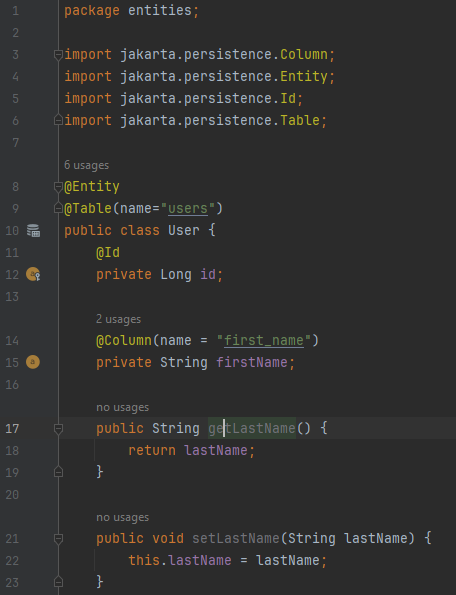
\includegraphics[width=6cm]{img/entity_class.png}
		};
	\end{tikzpicture}
	\begin{itemize}
		\item \texttt{@Table} : nom table
		\item \texttt{@Id} : associer un attribut \\de la classe à la clé primaire
		\item On peut ajouter l'annotation\\ suivante à l'attribut annoté\\ @Id si jamais les clés sont\\ générées par la BdD:\\
		{\footnotesize\texttt{@GeneratedValue(strategy =\\ GenerationType.AUTO)}}
		\item \texttt{@Column} : associer un attribut\\ à une colonne dans la table
		\item[*] Noter l'élément \texttt{name} \\des annotations
		\vspace{1cm}
	\end{itemize}
\end{frame}


\begin{frame}
	\frametitle{Classe d'objets persistants -- contraintes}
	La classe annotée \texttt{@Entity} :
	\begin{itemize}
		\item doit posséder un constructeur vide, public ou protected. Pour rappel : ce constructeur vide existe par défaut si aucun constructeur n'existe dans la classe. Dans le cas contraire, il doit être ajouté explicitement;
		\item ne doit pas être \texttt{final}, et aucune de ses méthodes ne peut être déclarée \texttt{final};
		\item ne peut pas être une interface ou une énumération;
		\item peut être une classe concrète ou abstraite.
	\end{itemize}
\end{frame}


\begin{frame}
	\frametitle{Configuration de l'unité de persistance}
	\begin{tikzpicture}[overlay,remember picture]
		\node[anchor=center,xshift=0pt,yshift=20pt]
		at (current page.center) {
			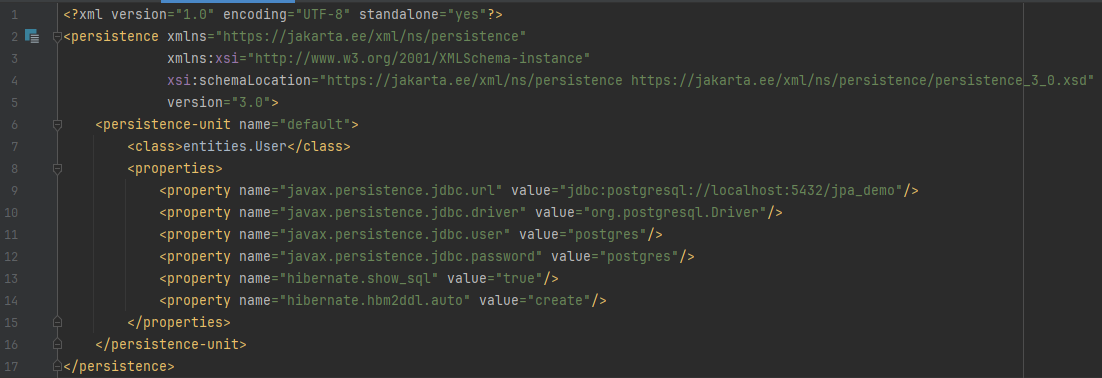
\includegraphics[width=12.5cm]{img/persistence_xml.png}
		};
	\end{tikzpicture}
	\begin{itemize}
		\vspace{4cm}
		\item Seules les deux dernières properties (pas obligatoires) sont spécifiques à l'implémentation de JPA Hibernate
		\item L'avant-dernière property permet de voir les requêtes SQL exécutées
		\item La dernière property permet de créer des records s'ils n'existent pas dans les tables
	\end{itemize}
	
\end{frame}

\begin{frame}
	\frametitle{Utiliser l'unité de persistance}
	\begin{tikzpicture}[overlay,remember picture]
		\node[anchor=center,xshift=0pt,yshift=-20pt]
		at (current page.center) {
			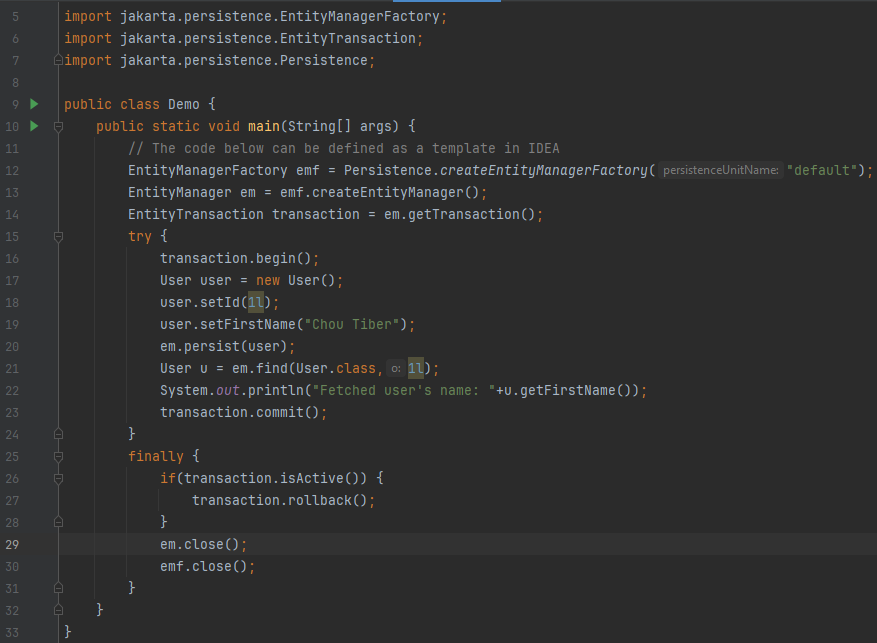
\includegraphics[width=10.5cm]{img/pu_usage.png}
		};
	\end{tikzpicture}
	
	
\end{frame}

\begin{frame}
	\frametitle{Opérations CRUD dans JPA}
	
	\begin{itemize}
		\item Création : \texttt{em.persist()}
		\item Mise à jour :  pas de méthode à invoquer pour mettre à jour une valeur en base. Dès qu'un objet est persistant, et que l'on modifie un de ses champs dans le cadre d'une transaction, alors sa valeur en base sera modifiée 
		\item Effacement : \texttt{em.remove()} en passant l'objet à supprimer en paramètre
		\item Recherche à partir d'une clé primaire : \texttt{em.find(...)}
	\end{itemize}
	
\end{frame}

\begin{frame}
	\frametitle{Annotations des attributs}
	
	\begin{itemize}
		\item  Les attributs d'une classe \texttt{@Entity} sont automatiquement associés à des colonnes en base, dans la table de l'entité
		\item Ces colonnes portent les mêmes noms que ces champs
		\item Si ces 2 règles s'appliquent, aucune annotation n'est nécessaire
		\item Les types associés automatiquement à des colonnes sont :
		\begin{itemize}
			\item Tous les types de base Java : int, long, float, etc...
			\item Tous les types enveloppes ( wrappers ) des types de base, et le type String;
			\item Les types date java.sql.Date, java.sql.Time et java.sql.TimeStamp. Les types java.util.Date et java.util.Calendar ne sont donc pas associés automatiquement;
			\item Les types énumérés;
			\item Les types Serializable, qui sont rangés dans des blob.
		\end{itemize}
		
	\end{itemize}
	
\end{frame}

\begin{frame}
	\frametitle{Annotation \texttt{@Column}}
	
	\begin{itemize}
		\item Annotation pouvant s'appliquer à un attribut ou à un getter
		\item Elle expose les attributs optionnels suivants :
		\begin{itemize}
			\item \texttt{name} : permet d'indiquer le nom de la colonne;
			\item \texttt{length} : pour les chaînes de caractères, cet attribut permet de fixer la taille du champ SQL associé. Cette taille n'est pas vérifiée dans le code Java;
			\item \texttt{unique} : ajoute une contrainte d'unicité sur la colonne;
			\item \texttt{nullable} : empêche cette colonne de porter des valeurs nulles. Cette contrainte est utile pour la définition de clés étrangères;
			\item \texttt{insertable}, \texttt{updatable} : empêche la modification des valeurs de cette colonne, utilisée pour les clés étrangères;
			\item ...
		\end{itemize}
		\item L'annotation \texttt{@Lob} permet de forcer l'application de cette colonne dans un blob SQL
	\end{itemize}
	
\end{frame}

\begin{frame}[fragile]
	\frametitle{Données de type temporel (dates, heures, ...)}
	
	\begin{itemize}
		\item  Les attributs de type \texttt{java.util.Date} et \texttt{java.util.Calendar} ne sont pas associés avec des données en base directement
		\item Pour préciser le type SQL, on utilise l'annotation \texttt{@Temporal}
		\item Cette annotation prend un unique élément :
		\begin{itemize}
			\item \texttt{TemporalType.DATE} : enregistre les dates en jour~/~mois~/~année ; 
			\item \texttt{TemporalType.TIME} : enregistre les dates en heure~:~minute~:~seconde ;
			\item \texttt{TemporalType.TIMESTAMP} : enregistre les deux informations de date et d'heure dans la journée
		\end{itemize}
		\item Exemple:
\begin{lstlisting}
@Column(name="date_de_naissance")
@Temporal(TemporalType.DATE)
private java.util.Date dateNaissance ;
\end{lstlisting}
	\end{itemize}
	
\end{frame}

\begin{frame}[fragile]
	\frametitle{Données de types énumération}
	
	\begin{itemize}
		\item  Les énumérations Java peuvent être associées à des colonnes de deux façons : 
		\begin{enumerate}
			\item Soit l'entity manager crée une colonne numérique, et stocke dedans un entier, qui correspond au numéro d'ordre de la valeur que porte le champ (efficace mais peu flexible), 
			\item Soit l'entity manager crée une colonne de type chaîne de caractères, et stocke le nom de la valeur énumérée.
		\end{enumerate} 
		\item On spécifie ce point avec l'annotation \texttt{@Enumerated}, qui peut prendre deux valeurs en attribut : \texttt{EnumType.ORDINAL} ou \texttt{EnumType.STRING}
		\item Exemple
\begin{lstlisting}
@Column(name="civility")
@Enumerated(EnumType.STRING)
private Civility civilite ;
\end{lstlisting}
	\end{itemize}
	
\end{frame}

\begin{frame}
	\frametitle{Opérations sur les entités}
	Toutes les opérations sur les entities passent par l'entity manager :
	\begin{itemize}
		\item  \texttt{persist}: rendre une entité persistante, c'est à dire l'écrire en base sur le prochain commit de la transaction dans laquelle on appelle persist;
		\item \texttt{remove}: rendre une entité non persistante, c'est à dire l'effacer de la base sur le prochain commit de la transaction dans laquelle on appelle remove;
		\item \texttt{refresh}: synchroniser l'état d'une entité avec son état en base. Si les champs d'une entité ont été modifiés dans la transaction courante, ces modifications seront donc effacées par cette opération. Si l'entité a été modifiée en base, alors ces modifications seront prises en compte lors d'un refresh;
	\end{itemize}

\end{frame}

\begin{frame}
\frametitle{Opérations sur les entités -- suite}	
	\begin{itemize}
		\item \texttt{detach}: détacher l'entité de l'entity manager qui la gère. Cette entité persistante ne sera donc pas prise en compte lors du prochain commit de la transaction dans laquelle on appelle detach;
		\item \texttt{merge}: attache l'entité à l'entity manager courant. On utilise cette opération pour associer une entité à un autre entity manager que celui qui a été utilisé pour la créer ou la lire.
	\end{itemize}	
\end{frame}

\section{Relations entre objets persistants}

\begin{frame}
	\frametitle{Mise en relation des entités}
	
	\begin{itemize}
		\item On peut définir quatre types de relations entre entités JPA :
		\begin{enumerate}
			\item relation 1:1 : annotée par \texttt{@OneToOne} ;
			\item relation n:1 : annotée par \texttt{@ManyToOne} ;
			\item relation 1:p : annotée par \texttt{@OneToMany} ;
			\item relation n:p : annotée par \texttt{@ManyToMany}.
		\end{enumerate}
		
		\item Les relations peuvent être unidirectionnelles ou bidirectionnelles
		\item Dans les relations bidirectionnelles, l'une des entités doit être maître et l'autre esclave
		
		\item Dans le cas des relations 1:1 et n:p, on peut choisir le côté maître comme on le souhaite
		
		\item Dans les relations 1:p et n:1, l'entité du côté 1 est l'entité esclave
		
	\end{itemize}
	
\end{frame}

\begin{frame}
	\frametitle{Relations 1:1}
	
	\begin{itemize}
		\item Relation entre Patient et CarteVitale
		\item Cas unidirectionnel : 
		\begin{itemize}
			\item l'entité Patient comporte un attribut de type CarteVitale annoté \texttt{@OneToOne}
			\item dans la BdD, la table Patient contient une colonne \texttt{num\_secu} qui est une clé étrangère
		\end{itemize}
		
		\item Cas bidirectionnel : l'entité esclave (CarteVitale) doit préciser un champ retour par une annotation \texttt{@OneToOne} et un attribut \texttt{mappedBy}, qui doit référencer le champ qui porte la relation côté maître (Patient)
		
	\end{itemize}
	
\end{frame}

\begin{frame}[fragile]
	\frametitle{Relations 1:p}
	
	\begin{itemize}
		\item Relation entre Patient et Consultation 
		\item Une relation 1:p est caractérisée par un champ de type Collection dans la classe maître
		\item La classe esclave ne porte pas de relation retour. Cette relation peut être spécifiée soit par l'annotation \texttt{@OneToMany} ou \texttt{@ManyToMany}
\begin{lstlisting}
@OneToMany
private Collection<Consultation> consultations ;
\end{lstlisting}		
		\item Elle peut être unidirectionnelle ou bidirectionnelle. Dans ce second cas, le côté maître est obligatoirement le côté qui tient la relation monovaluée
	\end{itemize}

\end{frame}

\begin{frame}[fragile]
\frametitle{Relations 1:p -- suite}

\begin{itemize}
		\item JPA crée une table de jointure entre les deux tables (entités)
		\item Cette table de jointure porte une clé étrangère vers la clé primaire de la première table, et une clé étrangère vers la clé primaire de la deuxième table		
		\item Cas bidirectionnel :  on ajoute une relation p:1 dans la classe destination de la relation
		\item Dans ce cas : l'élément \texttt{mappedBy} est défini pour l'annotation \texttt{@OneToMany}, mais pas pour l'annotation \texttt{@ManyToOne}
\begin{lstlisting}
// Dans la classe Patient
@OneToMany(mappedBy="patient")
private Collection<Consultation> consultations ;
// Dans la classe Consultation
@ManyToOne
private Patient patient;
\end{lstlisting}		
	\end{itemize}
	
\end{frame}

\begin{frame}
	\frametitle{Autres relations}
	
	\begin{itemize}
		\item La relation bidirectionnelle p:1 est identique à celle (bidirectionnelle) 1:p
		\item Cas d'une relation unidirectionnelle : annotation \texttt{@ManyToOne} sur un attribut de l'entité source de la relation (patient, par exemple)
		\item  JPA crée une colonne de jointure dans la table Consultation, et une clé étrangère qui référence la clé primaire de la table Patient
		\item Pour les relations n:p (annotation \texttt{@ManyToMany}) JPA crée en base une table de jointure avec des clés étrangères
		\item C'est la présence de l'attribut \texttt{mappedBy} qui crée le caractère bidirectionnel de la relation
	\end{itemize}
	
\end{frame}

\begin{frame}[fragile]
	\frametitle{Comportement \texttt{cascade}}
	
	\begin{itemize}
		\item Comportement cascade : spécifier ce qui se passe pour une entité en relation d'une entité père, lorsque cette entité père subit une des opérations \texttt{detach}, \texttt{persist}, \texttt{remove}, ...
		\item Comportement cascade précisé par l'élément \texttt{cascade} des annotations : \texttt{@OneToOne}, \texttt{@OneToMany} et \texttt{@ManyToMany}
		\item Valeur de cet élément à choisir dans l'énumération \texttt{CascadeType}
		\item Valeurs possibles : \texttt{DETACH}, \texttt{MERGE}, \texttt{PERSIST}, \texttt{REMOVE}, \texttt{REFRESH}, et \texttt{ALL} (toutes les valeurs précédentes)
\begin{lstlisting}
@OneToOne(cascade={CascadeType.PERSIST, CascadeType.REMOVE})
private CarteVitale carte;
\end{lstlisting}
	\end{itemize}
	
\end{frame}

\begin{frame}[fragile]
	\frametitle{Chargement des entités et leurs relations depuis la BdD}
	
	\begin{itemize}
		\item Est-ce que les relations doivent être chargées en même temps que les entités ?
		\begin{itemize}
			\item[*] Est-ce qu'on laisse faire un seul \texttt{SELECT} avec jointure ou bien des \texttt{SELECT} distincts? 
		\end{itemize}
		\item Tout dépend de l'applicatif
		\item JPA nous permet d'indiquer la façon de charger avec l'élément \texttt{fetch} des annotations \texttt{@OneToOne}, ... :
		\begin{enumerate}
			\item \texttt{FetchType.LAZY} : la relation doit être chargée à la demande ;
			\item \texttt{FetchType.EAGER} : la relation doit être chargée en même temps que l'entité qui la porte.
		\end{enumerate}
\begin{lstlisting}
@OneToMany(fetch=FetchType.EAGER)  // la relation est chargee par defaut
private Collection<Consultation> consultations ;
\end{lstlisting}		
	\end{itemize}
	
\end{frame}

\begin{frame}
	\frametitle{Optimisations possibles}
	
	\begin{itemize}
		\item  Annotation \texttt{@Embeddable} au lieu de \texttt{@Entity} (et \texttt{@Embedded} au lieu de \texttt{@Column}) pour ne pas multipler les tables de jointure
		\begin{itemize}
			\item[-] Cas d'une \texttt{Adresse} d'un \texttt{User}, par exemple 
			\item[-] On peut utiliser des \textit{Records} Java 16+ au lieu des classes
		\end{itemize}
		\item Annotations pour gérer les relations multivaluées particulières :
		\begin{itemize}
			\item \texttt{@OrderBy} ou \texttt{@OrderColumn} pour les java.util.List
			\item \texttt{@MapKeyColumn} pour les java.util.Map
		\end{itemize}
				
		\item Gestion de l'héritage entre classes dans le modèle relationnel (stratégies \texttt{SINGLE\_TABLE}, \texttt{JOINED} et \texttt{TABLE\_PER\_CLASS} -- voir cours BdD avancées)
		\item Langage de req. indépendant des BdD : JPQL (\textit{Java Persistence Query Language}) pour écrire des méthodes spécifiques
	\end{itemize}
	
\end{frame}

\begin{frame}
	\frametitle{Utiliser JPA dans IntelliJ IDEA}
	
	\begin{itemize}
		\item Lire le tuto :
		\url{https://www.youtube.com/watch?v=QJddHc41xrM}
		\item Le code adapté à Postgres est fourni sur le dépôt Moodle
	\end{itemize}
\end{frame}

\rquestionslide

\end{document}
